\documentclass[14pt]{extarticle}
\usepackage[margin=0.7in]{geometry}
\usepackage{tikz}
\usetikzlibrary{shadings}
\usepackage{fontawesome5}
\usepackage[T1]{fontenc}
\usepackage[default]{comicneue}
\usepackage{enumitem}
\pagestyle{empty}
\setlength{\parindent}{0pt}
\setlength{\parskip}{6pt}

% ---------- Pictures ----------
% A stone
\newcommand{\stone}[2]{\draw[line width=1.2pt] (#1,#2) circle (0.32);}

% A pile of #3 stones, in rows of 3, starting at (#1,#2)
\newcommand{\pile}[3]{%
  \foreach \i in {1,...,#3} {
    \pgfmathtruncatemacro{\col}{mod(\i-1,3)}
    \pgfmathtruncatemacro{\row}{(\i-1)/3}
    \stone{#1+0.75*\col}{#2+0.75*\row}
  }%
}

% A cookie
\newcommand{\cookie}[2]{%
  \fill[brown!60!orange!80, draw=brown!70!black, line width=1pt] (#1,#2) circle (0.55);
  \foreach \dx/\dy in {-0.25/0.2, 0.15/0.3, 0.25/-0.15, -0.1/-0.25, 0.0/0.05}
    \fill[brown!40!black] (#1+\dx,#2+\dy) circle (0.07);
}

% Big game title
\newcommand{\game}[1]{%
  \vspace{4pt}
  {\LARGE\bfseries #1}\par
  \vspace{2pt}
}

\newenvironment{rules}{\begin{itemize}[leftmargin=0pt, itemsep=2pt, topsep=2pt, label={}]\Large}{\end{itemize}}

% Rules on the left (#1 wide), picture on the right (the rest)
\newcommand{\beside}[3]{%
  \noindent\begin{minipage}[c]{#1}\raggedright #2\end{minipage}\hfill
  \begin{minipage}[c]{\dimexpr\linewidth-#1-4mm}\centering #3\end{minipage}\par
}

\begin{document}
\sffamily

\begin{center}
  {\Huge\bfseries More Nim Games}
\end{center}

%-------------------------------------------------
\game{Don't take the last stone!}
\begin{rules}
  \item Take 1, 2, or 3 stones.
  \item If you take the \textbf{last} stone, you \textbf{lose}!
\end{rules}
\begin{center}
\begin{tikzpicture}
  \foreach \i in {0,...,14} { \draw[line width=1.2pt] (0.8*\i,0) circle (0.34); }
  \node[font=\small] at (0,0) {\faSkull};
\end{tikzpicture}\\[2pt]
{\large 15 stones}
\end{center}

%-------------------------------------------------
\game{Nim with a cookie}
\begin{rules}
  \item Take 1, 2, or 3 stones.
  \item \textbf{Or} eat the cookie. Then you skip your turn!
  \item Only one player can eat the cookie.
  \item Take the last stone to win.
\end{rules}
\begin{center}

\begin{tikzpicture}
  \foreach \i in {0,...,9} { \stone{0.8*\i}{0} }
  \cookie{9.6}{0}
\end{tikzpicture}\\[2pt]
{\large 10 stones \ and \ 1 cookie}
\end{center}

\vspace{10pt}
%-------------------------------------------------
\game{Two Piles: 9 and 9}
\beside{11.2cm}{%
\begin{rules}
  \item Take 1, 2, or 3 stones from \textbf{one} pile.
  \item Take the last stone to win.
\end{rules}
}{%
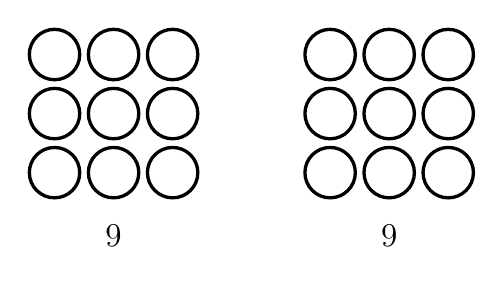
\begin{tikzpicture}
  \pile{0}{0}{9}
  \pile{3.5}{0}{9}
  \node[font=\large] at (0.75,-0.8) {9};
  \node[font=\large] at (4.25,-0.8) {9};
\end{tikzpicture}
}

\vspace{10pt}
%-------------------------------------------------
\game{Two Piles: 9 and 8}
\beside{11.2cm}{%
\begin{rules}
  \item Take 1, 2, or 3 stones from \textbf{one} pile.
  \item Take the last stone to win.
\end{rules}
}{%
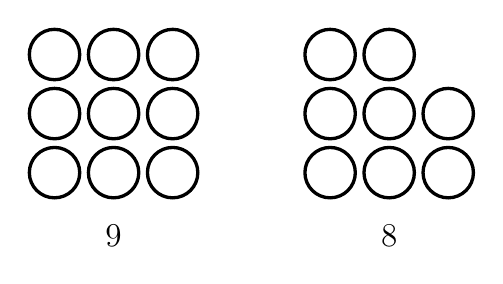
\begin{tikzpicture}
  \pile{0}{0}{9}
  \pile{3.5}{0}{8}
  \node[font=\large] at (0.75,-0.8) {9};
  \node[font=\large] at (4.25,-0.8) {8};
\end{tikzpicture}
}

\newpage
%-------------------------------------------------
\game{Three Piles: 7, 8, and 9}
\beside{9cm}{%
\begin{rules}
  \item Take as many stones as you like from \textbf{one} pile.
  \item Take the last stone to win.
\end{rules}
}{%
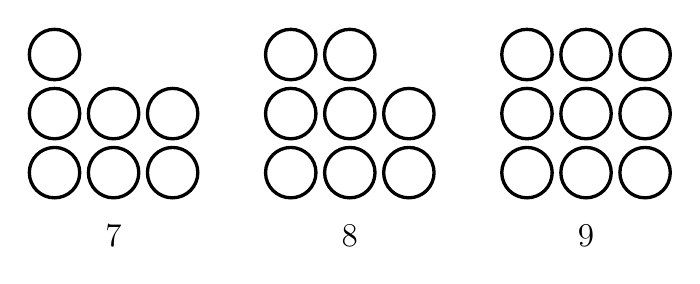
\begin{tikzpicture}
  \pile{0}{0}{7}
  \pile{3}{0}{8}
  \pile{6}{0}{9}
  \node[font=\large] at (0.75,-0.8) {7};
  \node[font=\large] at (3.75,-0.8) {8};
  \node[font=\large] at (6.75,-0.8) {9};
\end{tikzpicture}
}

\vspace{24pt}
%-------------------------------------------------
\game{Circle Nim}
\beside{12.8cm}{%
\begin{rules}
  \item Take 1 stone \textbf{or} take 2 stones that touch.
  \item Take the last stone to win.
\end{rules}
}{%
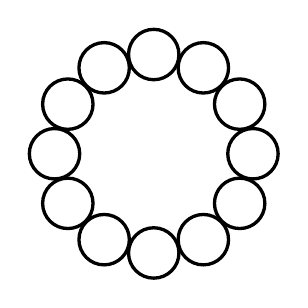
\begin{tikzpicture}
  \foreach \i in {0,...,11} { \stone{{1.26*cos(30*\i)}}{{1.26*sin(30*\i)}} }
\end{tikzpicture}\\[2pt]
{\large 12 stones}
}

\vspace{24pt}
%-------------------------------------------------
\game{Chomp the chocolate bar!}
\begin{rules}
  \item Pick a square. Eat it and \textbf{all} squares \textbf{up} and~to~the~\textbf{right}~of~it.
  \item The green square is poison. If you eat it, you \textbf{lose}!
\end{rules}
% Board on the left, example on the right
\begin{center}
\begin{minipage}[c]{8cm}
\centering
\begin{tikzpicture}[scale=1.5]
  % 5 wide, 4 tall
  \foreach \x in {0,...,4} \foreach \y in {0,...,3} {
    \fill[brown!55!black, rounded corners=2pt] (\x+0.04,\y+0.04) rectangle (\x+0.96,\y+0.96);
    \fill[brown!40!black, rounded corners=2pt] (\x+0.18,\y+0.18) rectangle (\x+0.82,\y+0.82);
  }
  % Yucky square
  \fill[green!60!black, rounded corners=2pt] (0.04,0.04) rectangle (0.96,0.96);
  \node[text=white, font=\Huge] at (0.5,0.5) {\faDizzy[regular]};
\end{tikzpicture}
\end{minipage}\hfill
\begin{minipage}[c]{9cm}
\centering
{\large\bfseries Example:} {\large If you pick the \faCheck\ square, you eat all the \faTimes\ squares too.}\par\vspace{8pt}
\begin{tikzpicture}[scale=0.9]
  \foreach \x in {0,...,4} \foreach \y in {0,...,3} {
    \fill[brown!55!black, rounded corners=2pt] (\x+0.04,\y+0.04) rectangle (\x+0.96,\y+0.96);
  }
  \fill[green!60!black, rounded corners=2pt] (0.04,0.04) rectangle (0.96,0.96);
  \foreach \x in {2,...,4} \foreach \y in {1,...,3} {
    \fill[white, opacity=0.55, rounded corners=2pt] (\x+0.04,\y+0.04) rectangle (\x+0.96,\y+0.96);
    \node[text=red!80!black, font=\large] at (\x+0.5,\y+0.5) {\faTimes};
  }
  \fill[yellow!80!orange, rounded corners=2pt] (2.04,1.04) rectangle (2.96,1.96);
  \node[text=blue!80!black, font=\Large] at (2.5,1.5) {\faCheck};
\end{tikzpicture}
\end{minipage}
\end{center}

\end{document}
